\documentclass[12pt,a4paper]{report}
\usepackage[T1]{fontenc}
\usepackage{graphicx}
\usepackage{amssymb, amsmath, amsthm}
\usepackage{xcolor}
\usepackage{nameref}
\usepackage{hyperref}
\usepackage{enumerate}
\usepackage{mdframed}

%\theoremstyle{definition}
%\newtheorem{question}{Question}
%
%\theoremstyle{remark}
%\newtheorem*{answer}{Answer}


\newcommand{\abs}[1]{|#1|}


\definecolor{QuestionColor}{RGB}{0, 115, 230} % Royal Blue
\definecolor{AnswerColor}{RGB}{0, 150, 136}   % Teal


\newtheoremstyle{blacknumbox} % Theorem style name
{0pt} % Space above
{0pt} % Space below
{\normalfont} % Body font
{} % Indent amount
{} % Theorem head font
{} % Punctuation after theorem head
{0.25em} % Space after theorem head
{\small\sffamily\bfseries\thmname{#1}~\thmnumber{#2} % Theorem text (e.g. Theorem 2.1)
	\thmnote{\sffamily\bfseries---~#3.\hspace{0.25em}}} % Optional theorem note

\theoremstyle{blacknumbox}
\newtheorem{corollaryT}{Question}

\newmdenv[
skipabove=7pt, % Whitespace above box
skipbelow=4pt, % Whitespace below box
rightline=false, % Right line visible
leftline=true, % Left line visible
topline=false, % Top line visible
bottomline=false, % Bottom line visible
linecolor=orange, % Line color
linewidth=4pt, % Line width
backgroundcolor=orange!5, % Background color
innerleftmargin=5pt, % Inside left margin width
innerrightmargin=5pt, % Inside right margin width
innertopmargin=5pt, % Inside top margin height
innerbottommargin=5pt, % Inside bottom margin height
leftmargin=0cm, % Outside left margin width
rightmargin=0cm % Outside right margin width
]{cBox}

\newenvironment{question}{\begin{cBox}\begin{corollaryT}}{\end{corollaryT}\end{cBox}}

\theoremstyle{blacknumbox}
\newtheorem*{answerT}{Answer}

\newmdenv[
skipabove=0pt, % Whitespace above box
skipbelow=10pt, % Whitespace below box
rightline=false, % Right line visible
leftline=true, % Left line visible
topline=false, % Top line visible
bottomline=false, % Bottom line visible
linecolor=cyan, % Line color
linewidth=4pt, % Line width
backgroundcolor=cyan!5, % Background color
innerleftmargin=5pt, % Inside left margin width
innerrightmargin=5pt, % Inside right margin width
innertopmargin=5pt, % Inside top margin height
innerbottommargin=5pt, % Inside bottom margin height
leftmargin=0cm, % Outside left margin width
rightmargin=0cm % Outside right margin width
]{answerBox}

\newenvironment{answer}{\begin{answerBox}\begin{answerT}}{\end{answerT}\end{answerBox}}



\begin{document}
	
	\begin{question} 
	If $A, B$ and $C$ are sets. prove the followings:
	\begin{enumerate}[(a)]
		\item $A \cap (B \cup C) = (A \cap B) \cup (A \cap C)$. \label{section-a}
		\item $C \textbackslash (A \cup B) = (C \textbackslash A) \cap (C \backslash B)$.
		
		\item $C \backslash (A \cap B) = (C \backslash A) \cup (C \backslash B) $.
		
	\end{enumerate}
	
	\begin{ans}
		\begin{enumerate}[(a)]
			\item 
			\begin{proof}
			Let $P, Q$, and $R$ be logical statements. We can show (using the truth table) that the following biconditional implication is a tautology. \[ P \wedge (Q \vee R) \Leftrightarrow (P \wedge Q) \vee (P \wedge R). \]
			Now let $x \in A \cap (B \cup C)$. Then $x \in A \wedge (x \in B \vee x \in C)$. Using the tautology above we can write $(x \in A \wedge x \in B) \vee (x \in A \wedge x \in C)$, thus $x \in (A \cap B) \cup (A \cap C) $, which means $A \cap (B \cap C) \subset (A \cap B) \cup (A \cap C)$. Conversely, let $x \in (A \cap B) \cup (A \cap C)$. By definition $(x \in A \wedge x \in B) \vee (x \in A \wedge x \in C)$. With the similar logic as above we can infer $(A \cap B) \cup (A \cap C) \subset A \cap (B \cup C)$. Thus $A \cap (B \cup C) = (A \cap B) \cup (A \cap C)$.
			\end{proof}
			
			\item 
			\begin{proof}
			Let $x \in C \backslash (A \cup B)$. By definition $x \in C \wedge x \notin (A \cup B) \biImp x \in C \wedge x \in \overline{A \cup B} \biImp x \in C \wedge x \in \bar{A} \cap \bar{B} \biImp x \in C \wedge (x \notin A \wedge x \notin B)$. Finally, using the following tautology 
			\[ P \wedge (Q \wedge R) \Leftrightarrow (P \wedge Q) \wedge (P \wedge R), \]
			we can write $(x \in C \wedge x \notin A) \wedge (x \in C \wedge x \notin B) \biImp x \in (C \backslash A) \cap (C \backslash B) $, thus $C \textbackslash (A \cup B) subset (C \textbackslash A) \cap (C \backslash B)$. The converse can be shown is true following the similar logic as below, thus inferring $C \textbackslash (A \cup B) = (C \textbackslash A) \cap (C \backslash B)$.
			\end{proof}
			
			\item \begin{proof}
			Let $x \in C \backslash (A \cap B)$. By definition $x \in C \wedge x \notin (A \cap B) \biImp x \in C \wedge x \in \overline{A \cap B} \biImp x \in C \wedge x \in \bar{A} \cup \bar{B} \biImp x \in C \wedge (x \notin A \vee x \notin B)$. Using the tautology in section (a),
			we can write $(x \in C \wedge x \notin A) \vee (x \in C \wedge x \notin B) \biImp x \in (C \backslash A) \cup (C \backslash B) $, thus $C \textbackslash (A \cap B) \subset (C \textbackslash A) \cup (C \backslash B)$. The converse can be shown is true following the similar logic as below, thus inferring $C \textbackslash (A \cap B) = (C \textbackslash A) \cup (C \backslash B)$.
			\end{proof}
			
			
			
			
		\end{enumerate}
	\end{ans}
\end{question}
	\begin{problem}
	There are 6 coins on a table, each showing heads (H) or tails (T). In each step we 
	\begin{itemize}
		\item Select uniformly one of the coins. 
		\item If it is heads, toss it and replace on the table (with random side).
		\item If it sis tails, toss it. If it comes up heads, leave it at that. If it comes up tails, toss it a second time, and leave the result as it is.
		Let $X_n$ be the number of heads showing after $n$ such steps. Answer the following questions
		\begin{enumerate}[(a)]
			\item Determine the transition probabilities for this Markov chain.
			\item Draw the transition diagram and write the transition matrix.
			\item What is $\prob(X_2 = 4| X_0=5)$?
		\end{enumerate}
	\end{itemize}
\end{problem}
\begin{solution}
	\begin{enumerate}[(a)]
		\item To compute the transition probabilities, we need to perform the first step analysis. Let the events \[I = \set{X_1 = a+1},\qquad S = \set{X_1 = a},\qquad D = \set{X_1 = a-1},\]
		where $0 \leq a \leq 6$ is the number of heads. So to compute the transition probabilities, we need to compute
		\[ P(a,a+1) = \prob_a(I), \qquad P(a,a) = \prob_a(S), \qquad P(a,a-1) = \prob_a(D). \]
		We start with $\prob_a(I)$. Let $ST$ be the event where the selected coin is tails, and $SH$ be the event where the selected coin is heads. These two events are disjoint and the probability of their union is 1, thus
		\[ \prob_a(I) = \underbrace{\prob_a(I|SH)}_{\text{see Eq (2.I.1)}}\underbrace{\prob_a(SH)}_{\frac{a}{6}} + \underbrace{\prob_a(I|ST)}_{\text{see Eq (2.I.2)}}\underbrace{\prob_a(ST)}_{\frac{6-a}{6}}. \tag{2.I}\]
		Note that if we start with $a$ coins heads, then the chance we choose a random coin from the table and find it heads is $\frac{a}{6}$, hence $\prob_a(SH) = \frac{a}{6}$, and $\prob_a(ST) = \frac{6-a}{6}$. Now we need to expand the remaining terms with appropriate conditioning. Let $TT$ be the event where we toss a coin and find it tails and $TH$ be the event where we toss a coin and find it heads. Thus we can write
		\[ \prob_a(I|SH) = \underbrace{\prob_a(I|SH,TH)}_{0}\underbrace{\prob_a(TS)}_\frac{1}{2} + \underbrace{\prob_a(I|SH,TT)}_{0}\underbrace{\prob_a(TT)}_\frac{1}{2}. \tag{2.I.1}  \]
		Note that $\prob_a(TT) = \prob_a(TH) = \frac{1}{2}$, since the coin tossing is fair. Also, note that $\prob_a(I|SH,TH)=\prob_a(I|SH,TT)=0$ since if we select a heads, and then toss it, finding it either heads or tails will not increase the total number of heads on the table. Similarly, for the other term in $(2.1)$ we have
		\[ \prob_a(I|ST) = \underbrace{\prob_a(I|ST,TH)}_{1}\underbrace{\prob_a(TH)}_{\frac{1}{2}} + \underbrace{\prob_a(I|ST,TT)}_\text{see Eq (2.I.3)}\underbrace{\prob_a(TT)}_{\frac{1}{2}}. \tag{2.I.2} \]
		Now we need to expand the remaining terms in the equation above.
		\[ \prob_a(I|ST,TT) = \underbrace{\prob_a(I|ST,TT,TH)}_{1}\prob_a(TH) + \underbrace{\prob_a(I|ST,TT,TT)}_{0}\prob_a(TT) = \frac{1}{2}. \tag{2.I.3}  \]
		Putting all together we can write
		\[ \boxed{P(a,a+1) = \prob_a(I) = \frac{6-a}{8}}. \]
		Similarly, we can compute other transition probabilities. For instance for $\prob_a(S)$ we can write
		\[ \prob_a(S) = \underbrace{\prob_a(S|SH)}_{\text{see Eq (2.S.1)}}\underbrace{\prob_a(SH)}_{\frac{a}{6}} + \underbrace{\prob_a(S|ST)}_{\text{see Eq (2.S.2)}}\underbrace{\prob_a(ST)}_{\frac{6-a}{6}}. \tag{2.S}\]
		and for the remaining terms we can write
		\[ \prob_a(S|SH) = \underbrace{\prob_a(S|SH,TH)}_{1}\underbrace{\prob_a(TS)}_\frac{1}{2} + \underbrace{\prob_a(S|SH,TT)}_{0}\underbrace{\prob_a(TT)}_\frac{1}{2}, \tag{2.S.1}  \]
		and
		\[ \prob_a(S|ST) = \underbrace{\prob_a(S|ST,TH)}_{0}\underbrace{\prob_a(TH)}_{\frac{1}{2}} + \underbrace{\prob_a(S|ST,TT)}_\text{see Eq (2.S.3)}\underbrace{\prob_a(TT)}_{\frac{1}{2}}. \tag{2.S.2} \]
		And for the remaining term above
		\[ \prob_a(S|ST,TT) = \underbrace{\prob_a(S|ST,TT,TH)}_{0}\prob_a(TH) + \underbrace{\prob_a(S|ST,TT,TT)}_{1}\prob_a(TT) = \frac{1}{2}. \tag{2.S.3}  \]
		and by putting all together we will get
		\[\boxed{ P(a,a) =  \prob_a(S) = \frac{6+a}{24}}. \]
		Finally, since $\prob_a(I\cup S \cup D) = 1$, and $I,S,D$ are mutually disjoint, we can write 
		\[ \prob_a(D) = 1 - (\prob_a(I) + \prob_a(S)), \] 
		hence
		\[ \boxed{P(a,a-1) = \prob_a(D) = \frac{a}{12}}. \]
		so the transition probabilities are as calculated.
		
		\item The transition diagram is plotted below. 
		
		\begin{center}
			\begin{tikzpicture}[->,>=stealth',shorten >=1pt,auto,node distance=1.9cm,
				semithick,scale=0.4]
				\tikzstyle{every state}=[circle, draw, fill=orange!50,
				inner sep=0pt, minimum width=10pt]
				
				\node[state] (A)              {$0$};
				\node[state]         (B) [right of=A] {$1$};
				\node[state]         (C) [right of=B] {$2$};
				\node[state]         (D) [right of=C] {$3$};
				\node[state]         (E) [right of=D] {$4$};
				\node[state]         (F) [right of=E] {$5$};
				\node[state]         (G) [right of=F] {$6$};
				
				\path (A) edge [bend left] node {$p_{01}$} (B)
				(B) edge [bend left] node {$p_{10}$} (A)
				(A) edge [loop left] node {$p_{00}$} (A)
 				
				(B) edge [bend left] node {$p_{12}$} (C)
				(B) edge [loop above] node {$p_{11}$} (C)
				(C) edge [bend left] node {$p_{21}$} (B)
				
				(C) edge [bend left] node {$p_{23}$} (D)
				(C) edge [loop below] node {$p_{22}$} (D)
				(D) edge [bend left] node {$p_{32}$} (C)
				
				(D) edge [bend left] node {$p_{34}$} (E)
				(D) edge [loop above] node {$p_{33}$} (E)
				(E) edge [bend left] node {$p_{43}$} (D)
				
				(E) edge [bend left] node {$p_{45}$} (F)
				(E) edge [loop below] node {$p_{44}$} (E)
				(F) edge [bend left] node {$p_{54}$} (E)
				
				(F) edge [bend left] node {$p_{56}$} (G)
				(F) edge [loop above] node {$p_{55}$} (E)
				(G) edge [bend left] node {$p_{65}$} (F)
				(G) edge [loop right] node {$p_{66}$} (G);
			\end{tikzpicture}
		\end{center}
		And the transition matrix is
		\[  M =
		\begin{pmatrix}
			1/4 & 3/4 & 0 & 0 & 0 & 0 & 0 \\
			1/12 & 7/24 & 5/8 & 0 & 0 & 0 & 0 \\
			0 & 1/6 & 1/3 & 1/2 & 0 & 0 & 0 \\
			0 & 0 & 1/4 & 3/8 & 3/8 & 0 & 0 \\
			0 & 0 & 0 & 1/3 & 5/12 & 1/4 & 0 \\
			0 & 0 & 0 & 0 & 5/12 & 11/24 & 1/8 \\
			0 & 0 & 0 & 0 & 0 & 1/2 & 1/2
		\end{pmatrix}
		 \]
		 
		 \item $\prob(X_2 = 4|X_0=5)$ is the second transition probability $P_2(5,4)$. To compute this, we need to fine the element in the 6-th row and 5-th column in the $M^2$ matrix, which is basically the inner product between the vectors formed by the 6-th row and the 5-th column.
		 \[ P_2(5,4) = (\frac{5}{12})^2 + \frac{11}{24}\cdot\frac{5}{12} = \frac{35}{96} \]
		 which after simplification becomes
		 \[ \boxed{P_2(5,4) = \frac{35}{96}}. \]
		\qed

		
		
		
	\end{enumerate}
	
\end{solution}
	\begin{question}
	A clock is broken. It has only one hand which moves every hour either clockwise with probability 1/2 or counter-clockwise with probability 1/2 (the numbers are from 0 to 11 and the hand moves by one full hour when it moves). Assume it starts at 0. What is the probability that it reaches 7 before coming back to 0 for the first time?
\end{question}
\begin{ans}
	First, let's draw the graph representing the state space of the random variable of interest.
	\begin{center}
		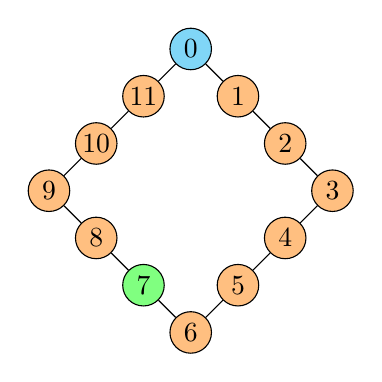
\begin{tikzpicture}[scale=0.6, every node/.style={circle, draw}]
			\tikzstyle{every node}=[circle, draw, fill=orange!50,
			inner sep=0pt, minimum width=15pt]
			
			
			\node[fill=cyan!50] (n0) at (0,3) {0};
			\node (n1) at (1,2) {1};
			\node (n2) at (2,1) {2};
			\node (n3) at (3,0) {3};
			\node (n4) at (2,-1) {4};
			\node (n5) at (1,-2) {5};
			\node (n6) at (0,-3) {6};
			
			\node (n11) at (-1,2) {11};
			\node (n10) at (-2,1) {10};
			\node (n9) at (-3,0) {9};
			\node (n8) at (-2,-1) {8};
			\node[fill=green!50] (n7) at (-1,-2) {7};
			
		
			\draw (n0) -- (n1);
			\draw (n1) -- (n2);
			\draw (n2) -- (n3);
			\draw (n3) -- (n4);
			\draw (n4) -- (n5);
			\draw (n5) -- (n6);
			\draw (n6) -- (n7);
			\draw (n7) -- (n8);
			\draw (n8) -- (n9);
			\draw (n9) -- (n10);
			\draw (n10) -- (n11);
			\draw (n11) -- (n0);
			
		\end{tikzpicture}
	\end{center}
	
	Define the event $B$ be $B = \set{T^+_0 > T_7}$. We are interested in finding $\prob_0(B)$. Now we can perform the first step argument as follows
	\[ p_0 = \frac{1}{2}(p_1 + p_{11}). \tag{3.1} \]
	Then we analyze each term in the right hand side of the equation above. For $p_1$ we have
	\[ \prob_1(B) = \underbrace{\prob_1(B|T_0>T_7)}_{1}\underbrace{\prob_1(T_0>T_7)}_{1/5} + \underbrace{\prob_1(B|T_0<T_7)}_{0}\underbrace{\prob_1(T_0<T_7)}_{6/7} = \frac{1}{5}. \]
	Note that $\prob_1(B|T_0>T_7)=1$ since it literally means the random walker reaches 7 before 0. Also $\prob_1(B|T_0<T_7)=0$ since the event $B$ is conditioned on reaching 0 before 7, which is clearly 0. The term $\prob_1(T_0>T_7)$ is computed using the Gambler's ruin analysis. Similarly, for the $p_{11}$ term we have
	\[ \prob_{11}(B) = \underbrace{\prob_{11}(B|T_0>T_7)}_{1}\underbrace{\prob_{11}(T_0>T_7)}_{1/7} + \underbrace{\prob_{11}(B|T_0<T_7)}_{0}\prob_{11}(T_0<T_7) = \frac{1}{7}. \]
	The rationale behind the values of the terms are the same as the ones discussed above. Now we can substitute everything in $(3.1)$
	\[ \boxed{p_0 = \frac{1}{2} (\frac{12}{35}) = \frac{6}{35}}. \]
	
\end{ans}
	\begin{question}
	The Fibonacci sequence is the sequence $(F_n)_{n\geq0}$ defined by $F_0 = 0, F_1=1$ and 
	\[ F_{n+2} = F_{n+1} + F_n \quad \text{for } n\geq 0.  \]
	Find a general formula for $F_n$
\end{question}
\begin{ans}
	First, we construct the characteristic polynomial of the sequence. From the recursive formula we can write
	\[ X^2 = X + 1 \implies \boxed{X^2 - X - 1 = 0}. \]
	The roots of the equation is 
	\[ r_1, r_2 = \frac{1 \pm \sqrt{5}}{2}. \]
	Now the general formula will be
	\[ F_n = Ar_1^n + Br_2^n. \] 
	To find the coefficients, we utilize the first two terms 
	\[ 0 = A + B, \qquad 1 = \frac{1}{2}(A+B) + \frac{\sqrt{5}}{2}(A-B). \]
	This system of equations implies that
	\[ A = \frac{1}{\sqrt{5}}, \qquad B=\frac{-1}{\sqrt{5}}.  \]
	Thus the general formula will be
	\[ \boxed{F_n = \frac{1}{\sqrt{5}}((\frac{1+\sqrt{5}}{2})^n - \frac{1-\sqrt{5}}{2})^n)}. \]
	
	\qed
	
\end{ans}
	\begin{question}
	Let $(X_n)$ be the simple random walk on the following graph. Compute $\prob_0(T_3<T_7)$.
	
	\begin{center}
		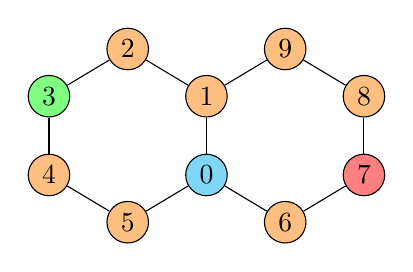
\begin{tikzpicture}[scale=1, every node/.style={circle, draw}]
			\tikzstyle{every node}=[circle, draw, fill=orange!50,
			inner sep=0pt, minimum width=15]
			
			
			\node[fill=cyan!50] (n0) at (0,0) {0};
			\node (n1) at (0,1) {1};
			\node (n2) at (-1,1.6) {2};
			\node[fill=green!50] (n3) at (-2,1) {3};
			\node (n4) at (-2,0) {4};
			\node (n5) at (-1,-0.6) {5};
			\node (n9) at (1,1.6) {9};
			\node (n8) at (2,1) {8};
			\node[fill=red!50] (n7) at (2,0) {7};
			\node (n6) at (1,-0.6) {6};

			\draw (n0) -- (n1);
			\draw (n1) -- (n2);
			\draw (n2) -- (n3);
			\draw (n3) -- (n4);
			\draw (n4) -- (n5);
			\draw (n5) -- (n0);
			\draw (n0) -- (n6);
			\draw (n6) -- (n7);
			\draw (n7) -- (n8);
			\draw (n8) -- (n9);
			\draw (n9) -- (n1);

			
		\end{tikzpicture}
	\end{center}
\end{question}
\begin{ans}
	For a much more simpler solution, let's define the two following notations
	\[ B = \{T_3 < T_7\}, \qquad p_v = \prob_v(B). \]
	Then, by first step argument at state $0$, we can write
	\[ p_0 = \frac{1}{3} (p_5 + p_6 + p_1).  \tag{5.1}\]
	Now we need to evaluate each of the terms in the right hand side. We start with $p_5$.
	\[ p_5 = \prob_5(B) = \underbrace{\prob_5(B|T_3<T_0)}_{1}\underbrace{\prob_5(T_3<T_0)}_{1/3} + \underbrace{\prob_5(B|T_3>T_0)}_{p_0}\underbrace{\prob_5(T_3>T_0)}_{2/3} = \frac{1}{3} + \frac{2}{3}p_0. \]
	note that $\prob_5(B|T_3<T_0) = 1$, since if we get to state 3, before getting to state 0, then it means that we have reached the state 3 before reaching the state 7, thus the event $B$ occurs with probability 1. Also $\prob_5(T_3<T_0) = 1/3$ from the Gambler's ruin. Furthermore $\prob_5(B|T_3>T_0) = p_0$ by using the Markov property, and finally $\prob_5(T_3>T_0) = 2/3$ by the Gambler's ruin. \\
	Now, we need to evaluate the term $p_6$. To analyze this term, we will do a first step argument starting at this point
	\[ p_6 = \prob_6(B) = \frac{1}{2}(\underbrace{p_7}_{0} + p_0) = \frac{p_0}{2}. \]
	Note that $p_7 = 0$, since then the event $B$ has not occurred. \\
	Finally, we need to analyze the term $p_1$. Again, by first step argument on this state we have
	\[ p_1 = \frac{1}{3}(p_0 + p_9 + p_2). \]	
	By doing a analysis on $p_9$ similar to the one we did for 5, we can write
	\[ p_9 = \prob_9(B)= \underbrace{\prob_9(B|T_7<T_1)}_{0}\prob_9(T_7<T_1) + \underbrace{\prob_9(B|T_7>T_1)}_{p_1}\underbrace{\prob_9(T_7>T_1)}_{2/3} = \frac{2}{3}p_1. \]
	The rationale behind the values for each term in the equation above, is exactly the same as in analyzing the terms of $p_5$.\\
	Now, we analyze the term $p_2$ by performing another first step analysis, similar to the one we did for state 6.
	\[ p_2 = \frac{1}{2}(\underbrace{p_3}_1 + p_1) = \frac{1}{2}(1+p_1). \]
	Now we can calculate $p_1$ in terms of $p_0$ which turns out to be
	\[ p_1 = \frac{6}{11}p_0 + \frac{3}{11}.  \]
	Now we insert all of the terms in the equation $(5.1)$ to get
	\begin{align*}
		&3p_0 = \frac{1}{3}+\frac{2}{3}p_0 + \frac{1}{2}p_0 + \frac{6}{11}p_0 + \frac{3}{11} \\ 
		&\implies 3p_0 - \frac{113}{66}p_0 = \frac{40}{33} \\
		&\implies p_0 = \frac{66}{85}\cdot\frac{40}{33} = \frac{16}{17}\\
		&\implies \boxed{p_0 = \frac{16}{17}}.
	\end{align*}


	\qed
	
	

\end{ans}
	\input{Q6.tex}
	\input{Q7.tex}
	\input{Q8.tex}
	\input{Q9.tex}
	\input{Q10.tex}
	

	
\end{document}